\uuid{4Bix}
\exo7id{7743}
\titre{exo7 7743}
\auteur{mourougane}
\organisation{exo7}
\datecreate{2021-08-11}
\isIndication{false}
\isCorrection{false}
\chapitre{Géométrie projective}
\sousChapitre{Géométrie projective}
\module{Algèbre et géométrie}
\niveau{L3}
\difficulte{}

\contenu{
\texte{
~

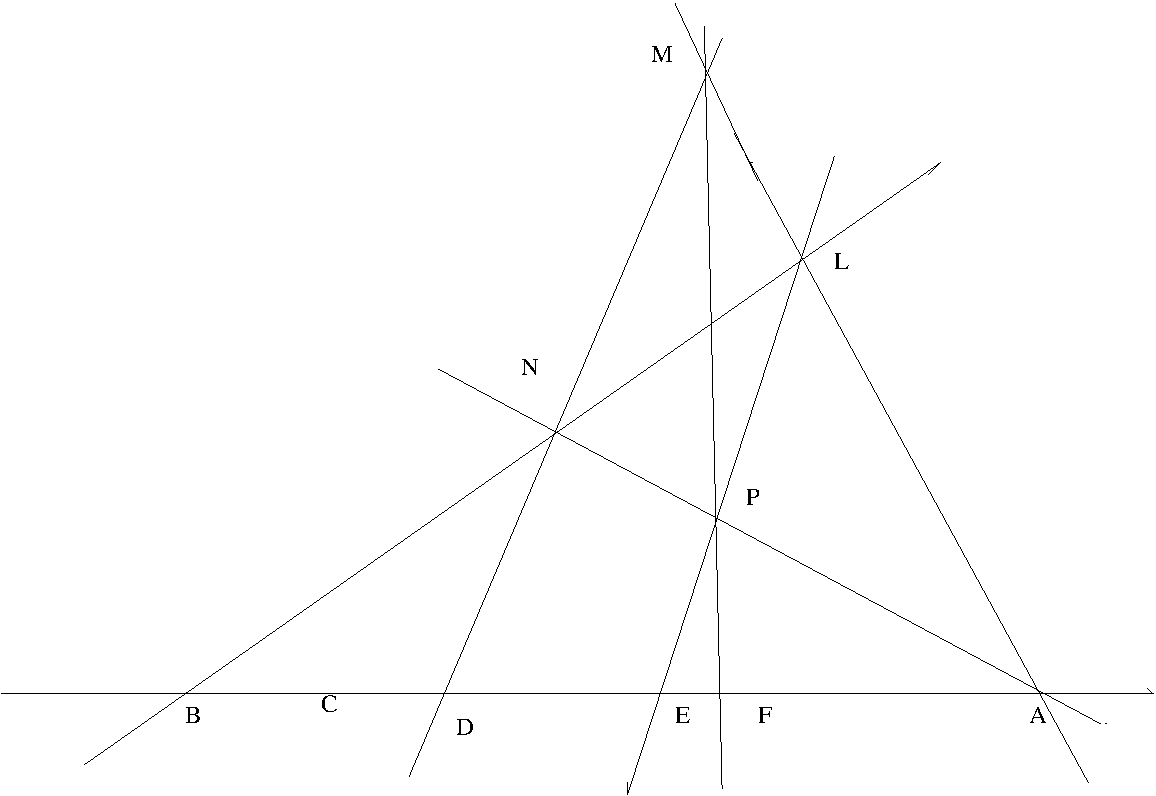
\includegraphics[scale=0.5]{images/4Bix-1}
}
\begin{enumerate}
    \item \question{Dessiner la configuration correspondante dans le plan affine $P(V)-(AM)$.}
    \item \question{Choisir des coordonnées homogènes telles que l’on ait $A = (1 : 0 : 0), B = (0 : 1 : 0), L = (0 : 0 : 1)
    $ et $ C = (1 : 1 : 0)$. Déterminer les équations des droites projectives $(BL), (DM), (NA), (LE), (MP)$ et les
    coordonnées homogènes des points $N = (BL) \cap (DM), P = (NA) \cap (LE)$ et $F = (AB) \cap (MP)$ en termes
    des coordonnées homogènes des points $D,E$ et $M$.}
    \item \question{Exprimer le birapport $[A,B,C,F]$ en termes de $x = [A,B,C,D]$ et $y = [A,B,C,E]$.}
\end{enumerate}
}
